%%
%% This is file `sample-acmsmall.tex',
%% generated with the docstrip utility.
%%
%% The original source files were:
%%
%% samples.dtx  (with options: `acmsmall')
%% 
%% IMPORTANT NOTICE:
%% 
%% For the copyright see the source file.
%% 
%% Any modified versions of this file must be renamed
%% with new filenames distinct from sample-acmsmall.tex.
%% 
%% For distribution of the original source see the terms
%% for copying and modification in the file samples.dtx.
%% 
%% This generated file may be distributed as long as the
%% original source files, as listed above, are part of the
%% same distribution. (The sources need not necessarily be
%% in the same archive or directory.)
%%
%% The first command in your LaTeX source must be the \documentclass command.
\documentclass[acmsmall]{acmart}
%\documentclass[manuscript,screen]{acmart}
\usepackage{multicol, caption}
\usepackage{placeins}

\newenvironment{Figure}
  {\par\medskip\noindent\minipage{\linewidth}}
  {\endminipage\par\medskip}


% NOTE that a single column version is required for submission and peer review. This can be done by changing the \doucmentclass[...]{acmart} in this template to 
%\documentclass[manuscript,screen]{acmart}

%%
%% \BibTeX command to typeset BibTeX logo in the docs
\AtBeginDocument{%
  \providecommand\BibTeX{{%
    \normalfont B\kern-0.5em{\scshape i\kern-0.25em b}\kern-0.8em\TeX}}}

%% Rights management information.  This information is sent to you
%% when you complete the rights form.  These commands have SAMPLE
%% values in them; it is your responsibility as an author to replace
%% the commands and values with those provided to you when you
%% complete the rights form.
\setcopyright{acmcopyright}
\copyrightyear{2020}
\acmYear{2020}
\acmDOI{10.1145/1122445.1122456}


%%
%% These commands are for a JOURNAL article.
\acmJournal{JACM}
\acmVolume{1}
\acmNumber{1}
\acmArticle{1}
\acmMonth{6}

%%
%% Submission ID.
%% Use this when submitting an article to a sponsored event. You'll
%% receive a unique submission ID from the organizers
%% of the event, and this ID should be used as the parameter to this command.
%%\acmSubmissionID{123-A56-BU3}

%%
%% The majority of ACM publications use numbered citations and
%% references.  The command \citestyle{authoryear} switches to the
%% "author year" style.
%%
%% If you are preparing content for an event
%% sponsored by ACM SIGGRAPH, you must use the "author year" style of
%% citations and references.
%% Uncommenting
%% the next command will enable that style.
%\citestyle{acmauthoryear}

%%
%% end of the preamble, start of the body of the document source.
\begin{document}


%%
%% The "title" command has an optional parameter,
%% allowing the author to define a "short title" to be used in page headers.
\title{caDDS: Community Assisted Distributed Database for Sequences}

%%
%% The "author" command and its associated commands are used to define
%% the authors and their affiliations.
%% Of note is the shared affiliation of the first two authors, and the
%% "authornote" and "authornotemark" commands
%% used to denote shared contribution to the research.
\author{El King Morado}
\authornote{Adviser}
\email{elkingmoradoking@gmail.com}
\affiliation{%
  \institution{University of the Philippines - Philippine Genome Center}
  \city{Quezon}
  \country{Philippines}
}

\author{Carl Araya}
\email{carl.araya256@gmail.com}
\affiliation{%
  \institution{University of the Philippines - Diliman}
  \city{Quezon}
  \country{Philippines}
}

\author{Jose Carlos Rodrigo J. Azcarraga}
\email{jjazcarraga@up.edu.ph}
\affiliation{%
  \institution{University of the Philippines - Diliman}
  \city{Quezon}
  \country{Philippines}
}


%%
%% By default, the full list of authors will be used in the page
%% headers. Often, this list is too long, and will overlap
%% other information printed in the page headers. This command allows
%% the author to define a more concise list
%% of authors' names for this purpose.
\renewcommand{\shortauthors}{Araya and Azcarraga}

%%
%% The abstract is a short summary of the work to be presented in the
%% article.
\begin{abstract}
Genomics data the past few years have grown exponentially with the technology barely keeping up. The problem faced by genome researchers is the large data set and difficulty transferring the files. Previous distributed databases are either not meant for genome data, or difficult to replicate. This paper lays the groundwork for a distributed database that is designed to easily scale to accommodate bigger storage, and also reduces the data speed bottleneck faced by centralized databases. The proposed system has a master node and data nodes. The master node handles administrative work while the Data nodes contain all sequence data. Data nodes should theoretically increase data transfer speeds. While current databases(e.g. NCBI) have more data, more users, and a live platform. The proposed system is aimed towards a smaller community, with more frequent and localized data, which the data storage can easily be expanded as the need arises. The proposed system is also theoretically faster as long as there are multiple working data nodes. A recommendation is to implement the system and make the code public for the use of other communities.
\end{abstract}

%%
%% The code below is generated by the tool at http://dl.acm.org/ccs.cfm.
%% Please copy and paste the code instead of the example below.
%%
\begin{CCSXML}
<ccs2012>
   <concept>
       <concept_id>10010405.10010444.10010093</concept_id>
       <concept_desc>Applied computing~Genomics</concept_desc>
       <concept_significance>500</concept_significance>
       </concept>
   <concept>
       <concept_id>10002951.10002952.10002953</concept_id>
       <concept_desc>Information systems~Database design and models</concept_desc>
       <concept_significance>500</concept_significance>
       </concept>
   <concept>
       <concept_id>10003120.10003130</concept_id>
       <concept_desc>Human-centered computing~Collaborative and social computing</concept_desc>
       <concept_significance>500</concept_significance>
       </concept>
 </ccs2012>
\end{CCSXML}

\ccsdesc[500]{Applied computing~Genomics}
\ccsdesc[500]{Information systems~Database design and models}
\ccsdesc[500]{Human-centered computing~Collaborative and social computing}

%%
%% Keywords. The author(s) should pick words that accurately describe
%% the work being presented. Separate the keywords with commas.
\keywords{genomics, distributed, database, community}


%%
%% This command processes the author and affiliation and title
%% information and builds the first part of the formatted document.
\maketitle

%%%%%%%%%%%%%%%%%%%%%%%%%%%%%%%%%%%%%%% INTRODUCTION %%%%%%%%%%%%%%%%%%%%%%%%%%%%%%%%%%%%%%%%%%%%%%%%%%%
\begin{multicols}{2}

\section{Introduction}

There is a vast amount of information inside the human body. One of these key biological information storage designs are in the genes. These tell each cell how to organize, how to build, and how to maintain the organism\cite{alberts_mole}. The genes inside a single cell (humans) when laid out is 2 meters in length.\cite{ency_sci_tech} And combining all of the cells, the information laid out would reach the moon, and back, 6000 times. 

These biological information storage designs or genes are studied in the field of \textit{Genomics}. Genomics studies the whole sets of genes and their interactions \cite[~p.437]{campbell}. The definition by the NIH (National Institute of Health) adds to that definition by including the study of how these genes interact with the environment.\cite{genomics-definition} Genes are large, the human genome specifically is filled with 3.2 billion pairs of information (or bases) \cite{introgenomics}.

Before these information are analyzed digitally, they must be read into a machine first. This is called \textit{Sequencing}. Here a machine takes fragments of genes and reads them into a digital format. These machines take in a lot of information from different but redundant fragments of genes to get a complete reading. Another set of computational processes are needed to combine these information to form the gene. Back in the 1980s the speed of sequencing was still slow and the top laboratory could only process around 1000 bases a day\cite{campbell}.

In 1993, when sequencing technology was still at its infancy. There was an initiative to complete the entire human genome\cite{introgenomics}. It was a slow process which took 10 years, a lot of collaborations, and 3 billion dollars. In 2000, when the human genome project had been ongoing, the speed of sequencing grew to processing 1000 base pairs every second, 24 hours a day, 7 days a week \cite{campbell}. The technology became faster and more reliable.

After the human genome project finished, there was a lot of data to be analyzed and many papers were published in the next few years. The research led to many advancements and many more genomes to be studied. From the whole genome of the closest relative to humans (chimpanzee) in 2006 to 4300 different whole genomes in 2013\cite[~p.442]{campbell}. Part of the reason why research was capable of looking at more whole genomes was because of next generation sequencing (NGS). NGS used a variety of technologies to make sequencing faster, cheaper, and more reliable\cite[~p.67]{paulselzer2018}. The technology speedup can be noticed in Japan, where today 10,000 human whole genomes can be studied in a single day. This has greatly increased the speed of research and data production in the field of genomics.

\begin{Figure}
\centering
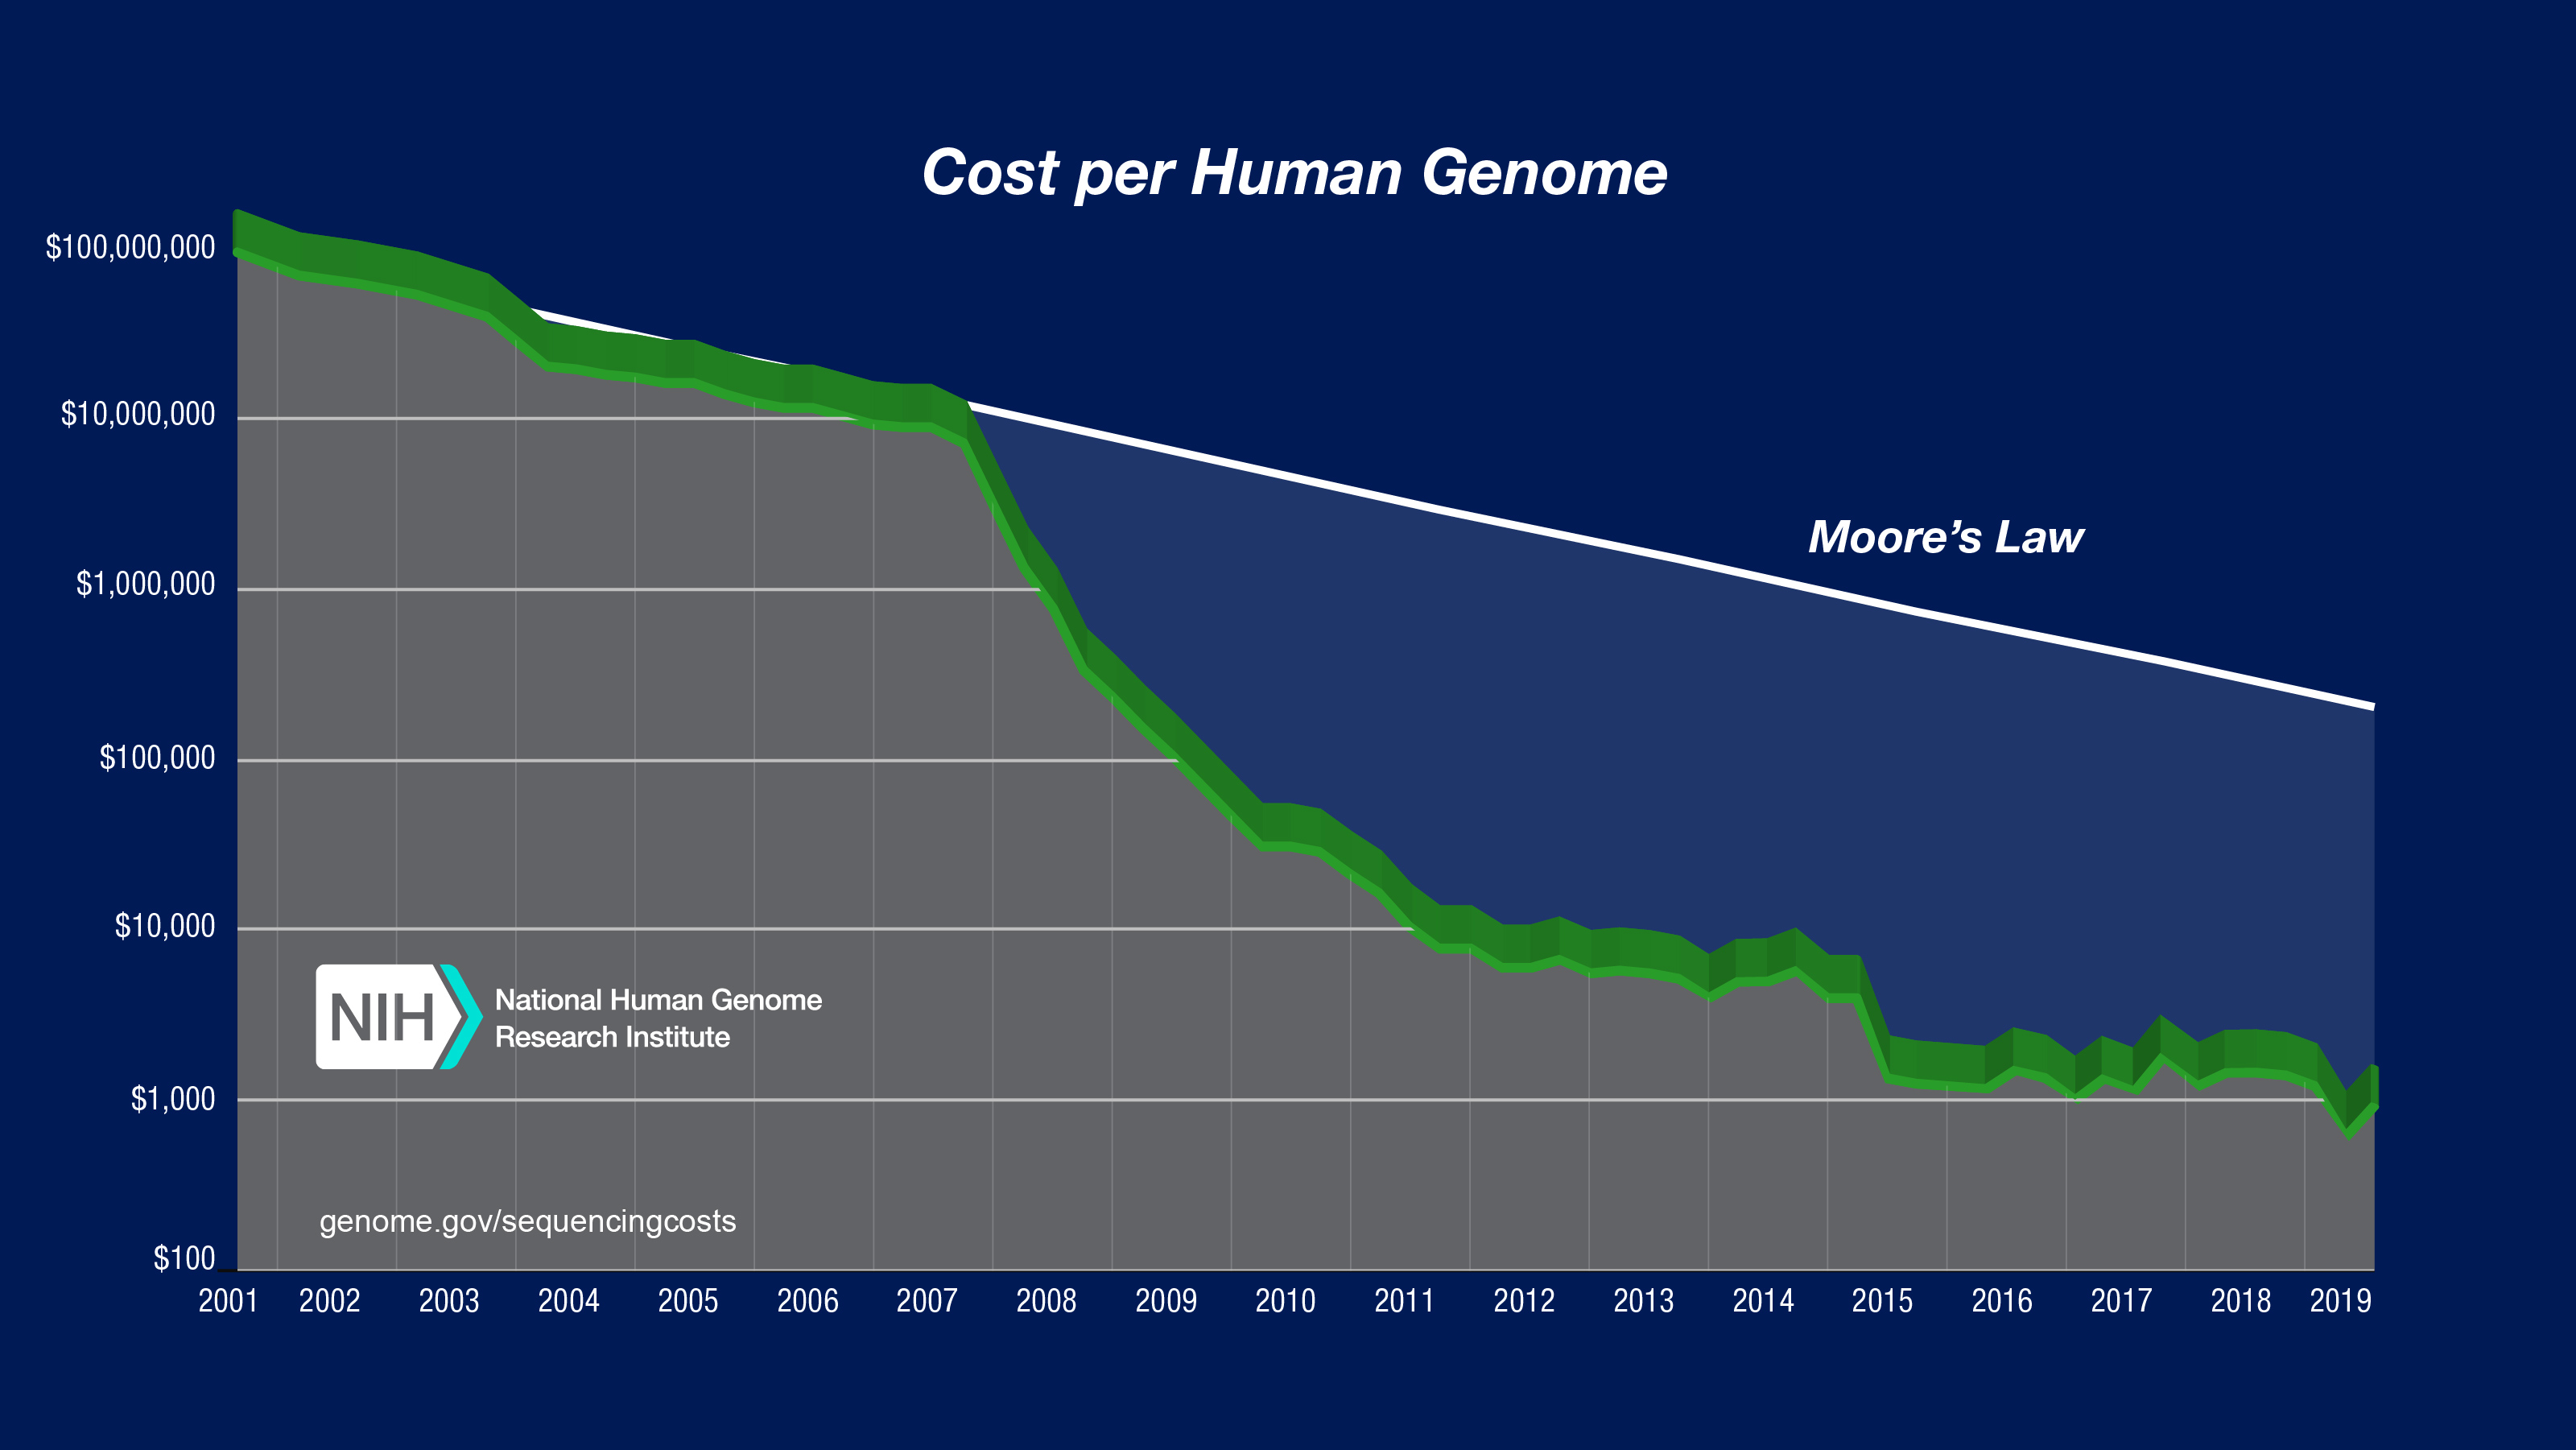
\includegraphics[width=0.80\linewidth]{images/human-gen-cost.jpg} 
\captionof{figure}{Cost per Genome Data Over Time}
\label{fig:human_gen_cost_fig}
\end{Figure}

\begin{Figure}
\captionof{figure}{Megabase Cost Over Time}
\centering
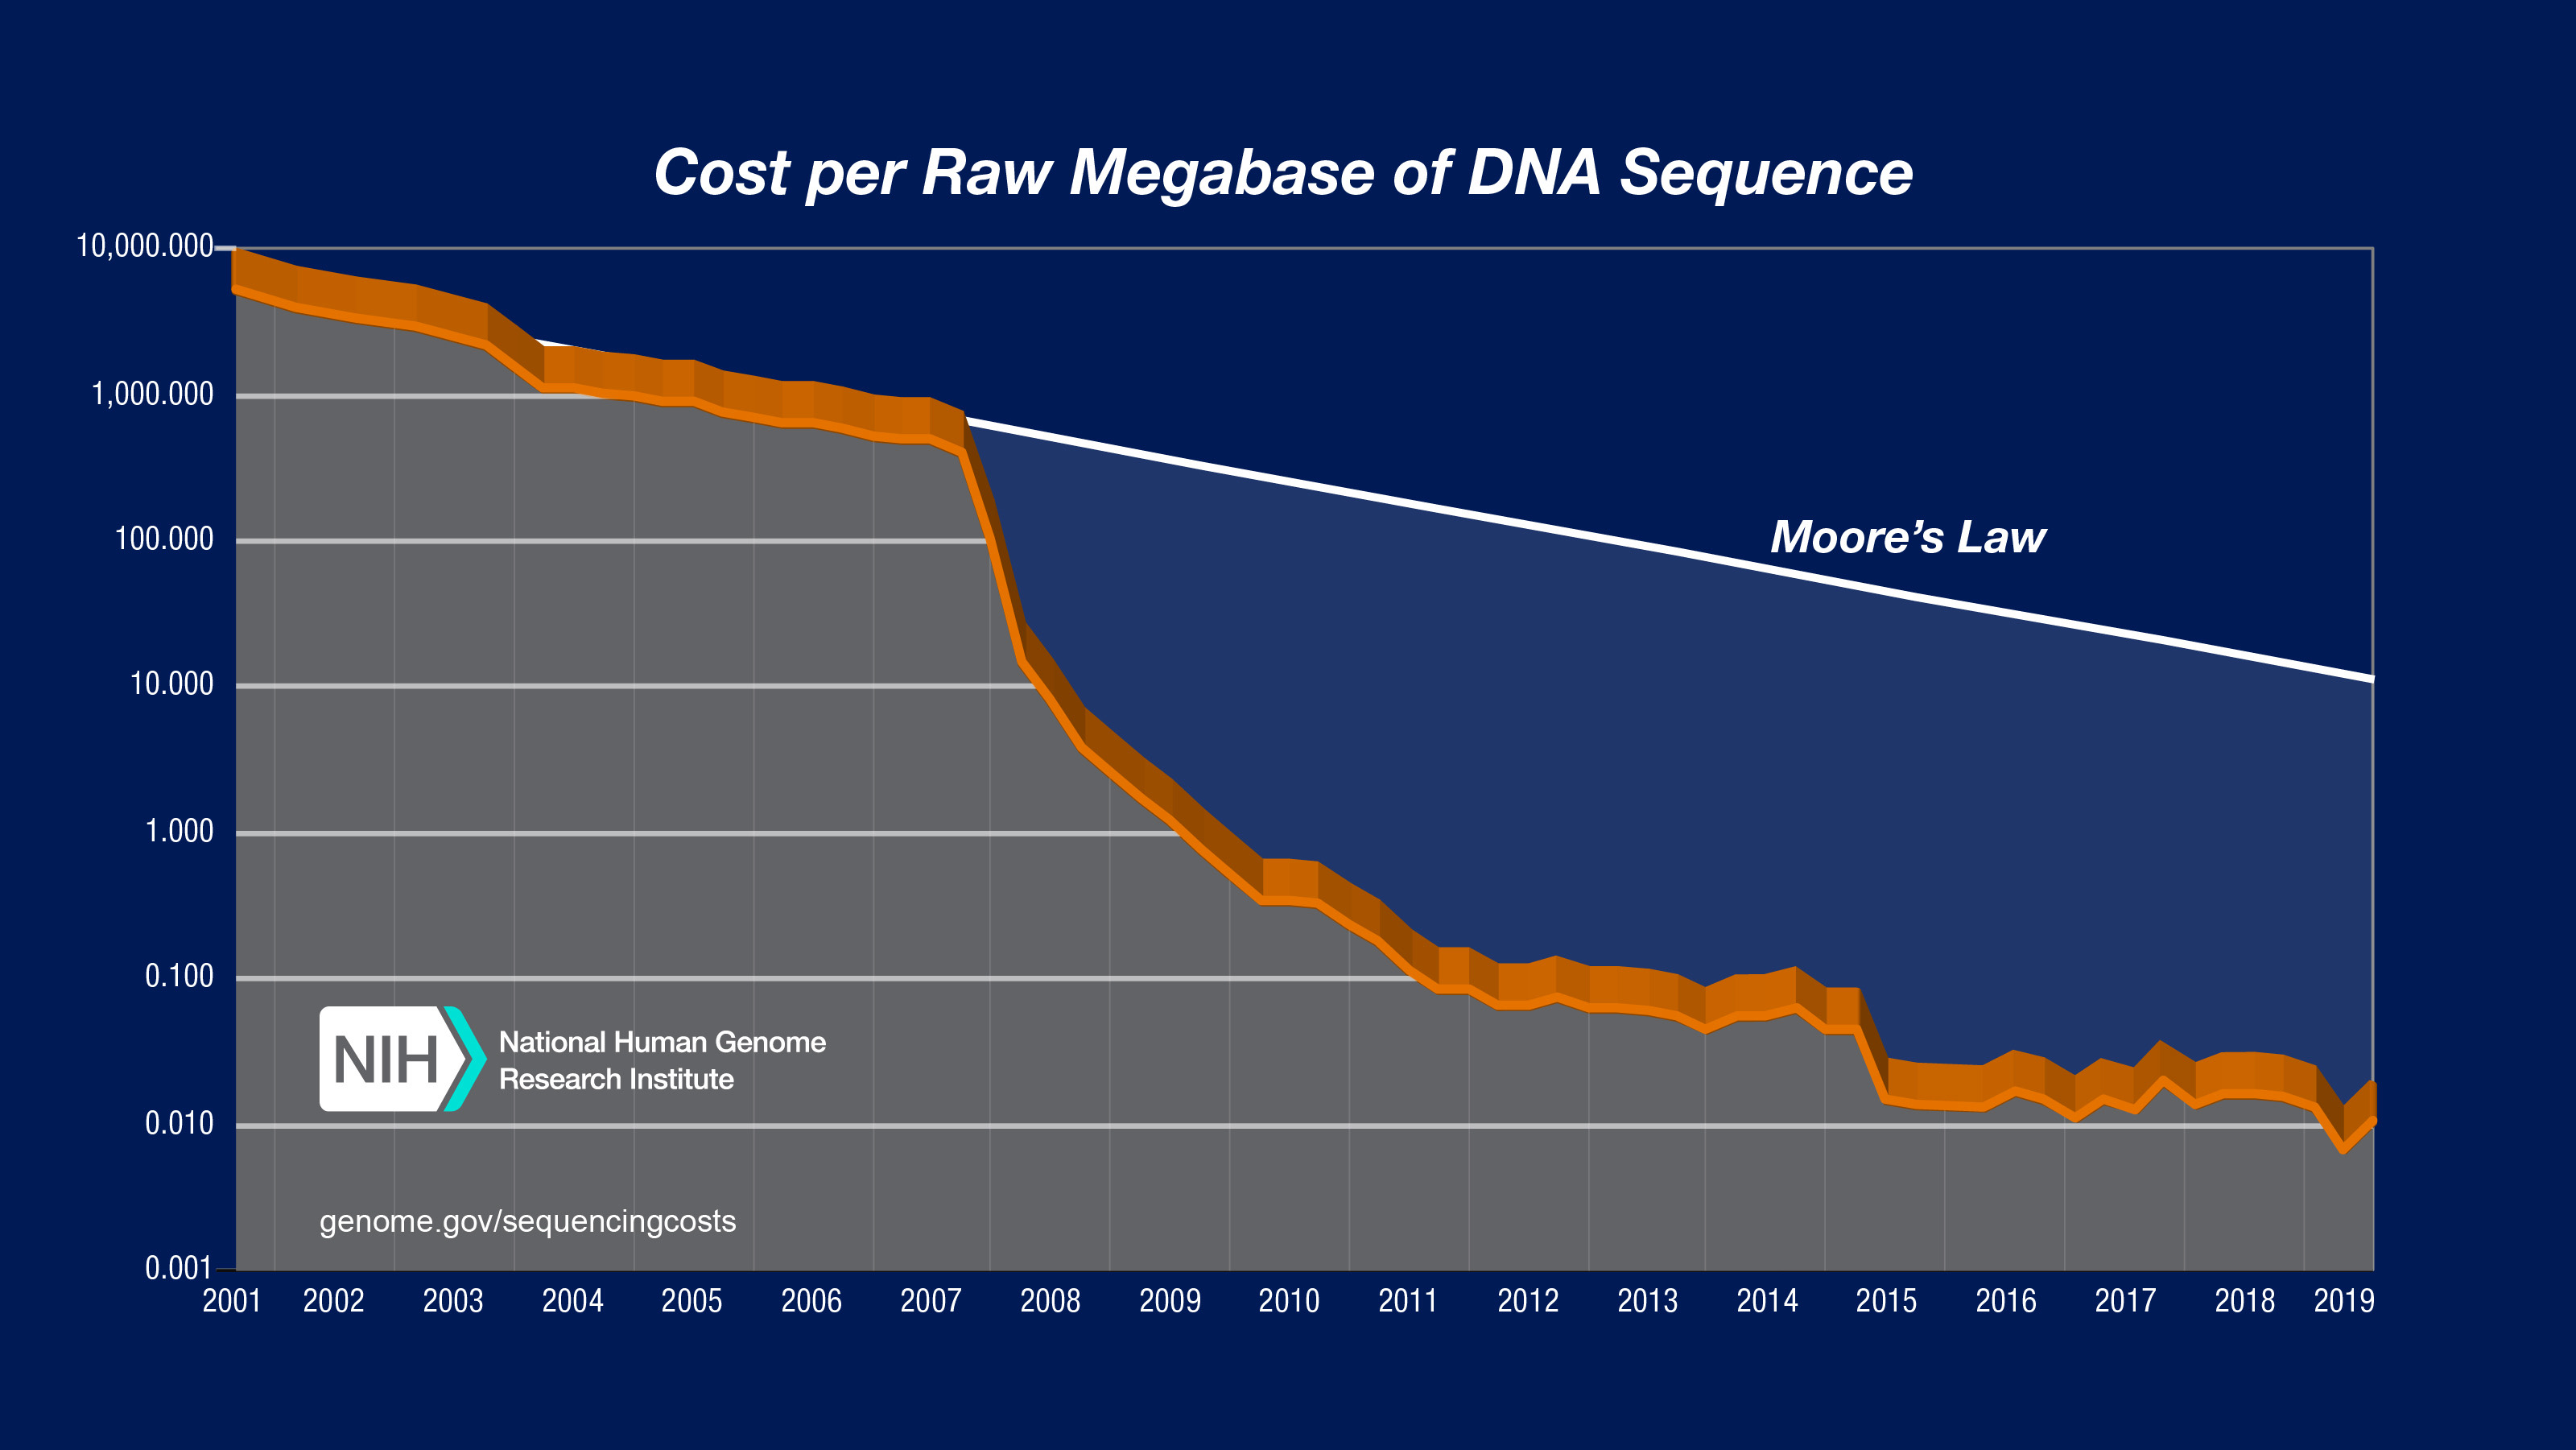
\includegraphics[width=0.80\linewidth]{images/seq-cost.jpeg} 
\label{fig:megabase_cost_fig}
\end{Figure}


In the Figure~\ref{fig:human_gen_cost_fig} \cite{genomics-cost}, it can be noticed that the cost per genome data goes down over time (note the year 2004-2005) where NGS was introduced. In this next Figure~\ref{fig:megabase_cost_fig}\cite{genomics-cost} we also note the drop of sequencing cost from 2008 to 2012 by 1000 fold \cite{bon_compression}. These graphs show how the cost has been reduced which should increase the data production by a huge amount as well.

The huge data must be stored in a form of digital information storage design as well. These are where the technologies of databases come in. Databases or DBMS (Database Management Systems) manage the digital information, and the access to it. \cite{Silberschatz2010}. The two types of databases are the centralized and the distributed databases\cite{centralizedvsdistributed}. The centralized databases have a single node or a single access point. While distributed databases have multiple nodes, and each node contains a portion or a replica of the data. Distributed databases are more complex but have higher availability, faster response, and are better for collaborative work. For genomics research, when the data storage needs to be increased often, distributed databases are most appropriate.

Databases also have three principles \cite{Silberschatz2010}, these 3 principles form the ideal database. But these 3 principles, practically cannot be done all at the same time \cite{Silberschatz2010}. These are the considerations and limitations that need to be addressed. One principle is consistency, data should be accurate and faithfully replicated. Another is availability, is the database able to serve users all of the time? The down times should be as infrequent as possible. The last and which will be the focus is Partition Tolerance. Partition Tolerance is the resiliency of a system. What happens when one portion malfunctions, will the whole system fail or will the rest easily adjust? This is necessary for a distributed database. And since Partition Tolerance \cite{Silberschatz2010} is chosen, then the trade off will be between availability and consistency.

The trade off for this system is between availability and consistency. For a consistency-priority-database, a change in one portion of the database, a create SQL command, will lock the entire database preventing other changes (reducing availability), then it will make sure that change is replicated in all relevant portions of the database, before making the database available again.

For an availability-priority-database, an example would be the messenger Facebook app. Where the focus of the app is speed. Here changes in a database will not lock the database, to make its app available. The downside is that the data is available, but it is not always up to date, and time is needed before the data is fully consistent on all the relevant databases.

%%%%%%%%%%%%%%%%%%%%%%%%%%%%%%%%%%%%%%% RRL %%%%%%%%%%%%%%%%%%%%%%%%%%%%%%%%%%%%%%%%%%%%%%%%%%%

\section{Review of Related Literature}

We review the technologies on data storage done before. Some have employed \textit{Client-Server}, some \textit{P2P}, others have tried \textit{Hybrid} (but are still few and unsuccessful).

\subsection{SeqTorr: A distributed scalable database for genomic information}
The focus on SeqTorr was finding a way to scale databases meant specifically for genomics information. There was also a focus on being able to choose information to share and use. The standard genomics workflow consists of uploading and downloading data on an international database like NCBI in Section \ref{NCBI}. Having a distributed scalable local infrastructure to store genomic data instead of relying on NCBI would be beneficial since: only certain sequences in NCBI are relevant to the institutions (e.g. Asian sequences are needed more than Caucasian ones), researchers within the country can share data with fast speeds,and institutions can share in the hosting of data.

The architecture of SeqTorr consists of a master node and multiple data nodes. The master node contains metadata of all the sequences and is where the user authentication is handled, while the data node is where the actual sequences are stored. All user uploads happen in the master node. When the master node receives a sequence from a user, it distributes the sequence to any available data nodes. 
\cite{seqtorr}

SeqTorr seems to go in the right direction to focus on genomics databases. But currently, SeqTorr is not available, and the code base does not have any documentation which makes future work on this difficult.

\subsection{BioTorrents}
BioTorrents focused on P2P and making it easy to share data across biological scientific communities. Scientific data continues to grow, and so does the demand for easier accessibility. Centralized servers, as stated earlier, which are using HTTP or FTP, cannot keep up with concurrent requests, and peer-to-peer protocols does not scale well for large files.\cite{biotorrents} One example of these centralized servers is NCBI, which will be discussed later. BitTorrent handles both these problems. 

BioTorrents is a system for legally sharing scientific data that works on top of the BitTorrent protocol (or P2P). It is much like a public tracker \cite{biotorrents}. The main website hosts torrent and metadata files. The main website doesn't store data, rather it lets the users keep the data and share it to other users. The main website only facilitates the sharing of these data (via the idea of P2P and torrents).

The main website stores info about each dataset includes categories, license, filenames, etc. that helps users in searching for relevant datasets. There is also a torrent file that has a list of trackers, servers that "know" which peers are serving which files, so it can download from those peers simultaneously. These torrents act like a directory telling the user who currently has the data for a piece of the file. The system then helps the user download many pieces of the file from many different users.

The client (or user) must have their computer continuously turned on to keep their file available to others. The main issue with BioTorrents, which is a problem as well in P2P, is that it requires lots of users to keep torrents available as often as possible.\cite{biotorrents} These entail that for the system to work, many people need to use it and all these people need to keep their computers on all the time.

BioTorrents was successful; many people had used it to share data. It was active for a while. However, BioTorrents has been down for years. This also shows what problems a system will face when doing a pure P2P application architecture.

\subsection{PeerDB}
% summarize intro
PeerDB is a proposed P2P system for sharing general data. Each node is equipped with a MySQL database that it keeps available for other nodes to download from. Each node also keeps track of its neighbors, and any useful information about them. Queries are passed around neighbors, with a maximum number of hops. A node may cache information about other peers to speed up future queries.
\cite{peerdb}

PeerDB is a proposal for a distributed system using P2P. For this to be used in the context of genomics biological work, a main website which facilitates sharing will be need to be put up. PeerDB needs to be installed as well on all the users who will be participating.

A future PeerDB system will also face similar problems faced by BioTorrents since it will need to rely on numerous active users for it to work.

\subsection{NCBI} \label{NCBI}
The National Center for Biotechnology Information or more commonly known as NCBI, which discussed briefly in the section on \textit{BioTorrents} and in the \textit{Introduction}, is the standard genomics database used by many researches and institutions. We will refer a portion of this later on as the \textit{base system}. This is the website used to access and store most genomics information around the world\cite{campbell}. It uses a client-server architecture. Users may download data via the graphics interface (website), or may be done via file transfer protocols such as FTP or HTTP \cite{biotorrents}. The latter is preferred since it may be done to automate the download of data.

The SeqTorr authors\cite{seqtorr} also stated that NCBI is the main and current DBMS used to get and share genomics data. But one difficulty using that is updating the current genomics dataset. There is currently no way to check which data (on your computer) have been updated, which sequences were corrected. And the way the authors solved this was to regularly re-download the entire NCBI database.

To state again some problems of NCBI, it has the limitations of \textit{Client-Server} architecture meaning the speed of the download is heavily reliant on the speed of the main NCBI server and the number of users accessing the server. Which also puts a lot of stress on the main server. Another problem discussed earlier was the updating of local user data, which have no technology yet to do so.



\begin{table*}[ht]
    \caption{Comparisons of Different Databases and Technologies}
    \label{table:database_comparison_table}
    \begin{tabular}{ccccc}
    \toprule
    System      & CS/P2P/H & Available? & DL/UL speed & Type of Data \\ 
    \midrule
    BioTorrents & P2P           & No         & Depends                    & Biological  \\ 
    SeqTorr     & H             & No         & Fast (PH server)           & Biological       \\ 
    PeerDB      & P2P           & No         & Depends                    & General      \\ 
    NCBI        & CS            & Yes        & Slow (US server)           & Biological  \\
    Dat Protocol    & P2P      & Yes        & Depends           & General  \\ 
    \bottomrule
    \end{tabular}
\end{table*} 

\subsection{Comparisons of Database Technologies} \label{compdb}

Table~\ref{table:database_comparison_table} compares the different technologies studied. An important point to note is that a majority of the databases are not available. This will also be used later on to describe what are the main problems of the different databases.

To restate the different gaps or problems found with other implementations of Genomic Databases: 
\subsection{Problems of Centralized Databases}
\begin{enumerate}
\item Genome researchers download an entire database of genomics data, especially when uncertain how to update their data
\item Genome researchers only need a portion of the database, but end up downloading the entire database
\item Client-Server approach can face bottlenecks (server speed) (Section \ref{client-server})
\item P2P approach has a need of a large unmoderated active user base to work (Section \ref{p2p})

\end{enumerate}

\subsection{Problems of Current Distributed Databases for Genomes}
\begin{enumerate}
    \item No existing usable public framework on distributed databases for genomes (Section \ref{compdb})
    \item Existing distributed database system for genomes is not replicable 
\end{enumerate}

\section{Problem}
To summarize the gaps described earlier, there are problems in implementations of centralized databases, specifically with bottlenecks and moderation. Other problems are specific to genome researchers with updating of the data. The last problem is the gap of usable distributed databases targeted towards genomics researchers. The main problem will be: "How to design a distributed database that is useful for genomics researchers?"

\section{Objectives}
Based on the problems we found described, we propose to:

\begin{itemize}
    \item Design the framework for an information system that speeds up the download and upload of genomics data
    \item  Design a distributed database system
    \item Evaluate the theoretical properties of the system based on the correctness and speed
\end{itemize}

The first objective addresses the genome researchers problems of centralized databases. The second objective aims to resolve the limitations of the client-server and P2P approaches, and the existing problems of distributed databases. The third objective aims to show the theoretical rationale for using these distributed databases. 


\section{Scope}

The research will focus on creating a theoretical design for the proposed system. And to evaluate the theoretical properties of the proposed system and the base system. The proposed system is the caDDS (community assisted Distributed Databases for Sequences), specifically the GET operation. While the base system, is the FTP (File Transfer Protocol) of NCBI for getting sequences. NCBI is currently a complex platform, but the scope of this research will only be the FTP access route.


\section{Limitations}
The research had time constraints and physical constraints because of the unexpected Covid-19 pandemic. The research will not implement the system or explain the technology stack to be used. It will not include security and authentication.


\section{Theoretical Framework}
Before the system features are discussed, notes about the design, and how it connects internally is needed to gain a better appreciation of the overall system


\subsection{Application Architecture}
The system's design is guided by the application architecture. Here it is discussed how an app that relies on networks functions and interacts \cite{kurose}. There are three main types: Client-Server, Peer-to-Peer, and Hybrid. Client-Server or CS means there is one web application that serves the data to multiple users (or clients, hence the name). As the number of clients grow bigger, the server takes more stress serving all the data. Peer-to-Peer or P2P is different since it has no singular dedicated server. No singular point of stress, and data is easily distributed. The term client and server is merged into a term "peer" that can both receive and send data. All peers can share data to other peers but the catch is that there is no centralized authority moderating these data, and that an active user base or peer base is needed for this to function.

Hybrid tackles some of the issues of CS and P2P, which is scalability and moderation. It allows easier scaling of database access (akin to adding more servers in P2P), but it also allows to have a form of moderation and security (akin to adding a moderator to CS). This is also more appropriate for a distributed database, and which is why a hybrid architecture is used.

\subsection{Dat Protocol}

The Dat Protocol is a newly-developed, open source peer-to-peer protocol for sharing data\cite{dat}. With a single command, anyone can start hosting a directory of files for others to download, as long as they have a publicly accessible IP address and port. Other users can download and then host their own copy of the same directory. Downloads are distributed, meaning if a file is shared across multiple active peers, a new user will be downloading that file from those peers, so bandwidth is shared, much like in BitTorrent. A file's data is synced across peers, so any changes made to the original copy of the file will be sent to peers hosting the same file. And like Git, the version history is also stored and made accessible to peers. Unlike Git though, Dat works well for any kind of file, not just source code. Dat also has security built in. Only users with the directory's read key can download it, and only users with the write key can make changes. In short, Dat has "taken the best parts of Git, BitTorrent, and Dropbox"\cite{dat}. Another important feature is that files and directories are stored as-is, meaning no modifications are done by Dat when storing files.

Dat's development began in 2013, so it is a relatively new protocol. There may still be large changes in the development and management of Dat, so the project is relatively volatile. Development is ongoing, and the community is active, yet there may still exist a few bugs and other difficulties when using Dat to build an application. Dat is built on NodeJS, and support for other programming languages and frameworks is quite limited. It also contains the same problems as other P2P protocols, namely, a lack of data moderation and incentives for users to serve as peers.


\subsection{Networks}
In each architecture it was discussed that there is a form of file transfer between peers or from servers to clients. To achieve this transfer, years of technology created systems called networks. There are 5 levels in a network \cite{kurose} but only the last 2, level 4 and 5 is needed for the system. The other levels 1-3 create protocols that send messages to specific and unique computers without error and utilizing any erratic medium between them (whether it be undersea cables or air). 
Level 4 assumes sending between computers is possible, but erratic. And these protocols in this level make sure all data is complete, error free before it is acknowledged. An important feature here is the File Transfer Protocol which is used by the NCBI. Here a client needs to set up a connection to the main NCBI server, then request specific files to be transferred to the client(or the user), and of course to move these files without error.

Level 5 abstracts level 4, and making the process of connecting and transferring easier to accomplish. Since Level 5 uses function calls to do the protocols of level 4. A designer of a system will want the ease-of-use of using level 5 functions, but will need knowledge of level 4 in order to better understand bugs and problems later on. Level 5 also allows the user to focus more on doing similar database or data manipulation functions (C.R.U.D.) as POST, GET, PUT, DELETE. 

All information systems must have POST, GET, PUT, DELETE or the corollary (C.R.U.D.). Since there are networks in this system, the network version of the data manipulation functions will be used.

\begin{itemize}
    \item The system being proposed is an information system, and this system will have the main API’s
    \begin{itemize}
        \item POST genome data
        \item GET genome data, this system will implement a hybrid P2P transfer
        \item PUT genome metadata (optional: PUT data)
        \item DELETE genome data
    \end{itemize}
\end{itemize}



\subsection{caDDS: Community Assisted Distributed Database for Sequences}

\subsubsection{Overview}
The two parts of the system infrastructure are the master node and data nodes. This system is also inspired by SeqTorr. 

The master node is a server that facilitates all authentication, uploading, and moderation. It also catalogs the metadata of all files. It will have a web application on top, with front-end and back-end that users wanting to upload a sequence to the system will have to access. The master node is also in charge of distributing sequence data to the data nodes.

The data nodes are servers that contain the sequence files themselves. Users will be downloading the sequences from these nodes. These nodes will also support the Dat protocol or a similar P2P network to enable instant syncing of data between data nodes and distributed download.

One institute will host the master node and be responsible for all system administration. This institute may also host a data node. Partner institutes will have their own data node/s that will share in the storage and distribution of sequences. Data nodes provide redundancy. The same sequence will be uploaded to multiple data nodes, so when a single data node becomes unavailable for whatever reason, no information is actually lost because copies have been made in other nodes. Data nodes also have the feature of enabling distributed download. Utilizing the P2P functionality provided by Dat, a researcher can download from multiple data nodes simultaneously, easing bandwidth requirements and speeding up transmission rate.

The system is essentially a database. The database stores sequence data. It has the normal CRUD functions meaning Create, Read, Update, Delete. It can let anyone download sequence data. But only registered users can upload sequence data. When a user uploads data, the moderator will verify the data's authenticity before allowing it to be uploaded. The master node will then contact data nodes and see which are available to host. 

Then for the downloading of the data. In the master node, the user will search for a sequence by keywords from its metadata. The user is then informed which currently available data nodes host the wanted sequence. The user will download normally from a single host using HTTP, or they can choose to download from multiple nodes simultaneously, with the P2P protocol described above.

% END OF ROUGH DRAFTS

The system is described as \textit{community assisted}. Since ideally, institutions can contribute to sharing the data by hosting servers that will become the data nodes. This sharing allows a greater bandwidth, and hopefully speed in which this data can be transferred. 

The database is a distributed database, which will aim to utilize the best features from peer-to-peer and client-server architectures. This will also aim to store sequences. Thus the "Distributed Database for Sequences" portion of the title.

Figure 3 shows the way in which the different components of the network interact with each other. The master node is connected to all data nodes for syncing purposes. 

\begin{Figure}
\captionof{figure}{App network diagram}
\centering
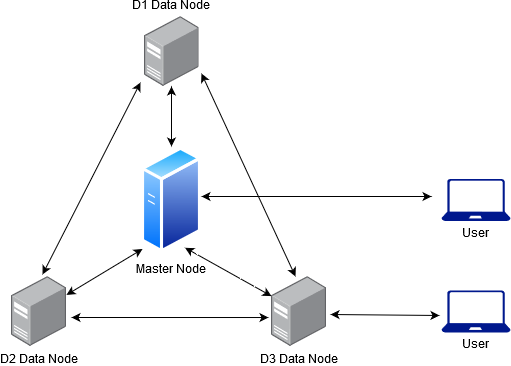
\includegraphics[width=0.8\linewidth]{images/thesis1.png} 
\end{Figure}

\begin{Figure}
\captionof{figure}{POST: Uploading a sequence}
\centering
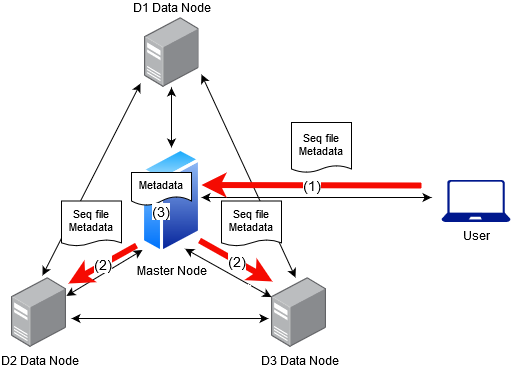
\includegraphics[width=0.80\linewidth]{images/thesis1-Page-3.png} 
\end{Figure}

\begin{Figure}
\captionof{figure}{GET: Downloading a sequence}
\centering
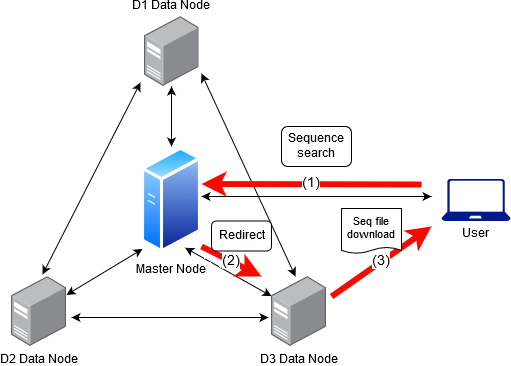
\includegraphics[width=0.80\linewidth]{images/thesis4.png} 
\end{Figure}

\begin{Figure}
\captionof{figure}{PUT: Updating a sequence}
\centering
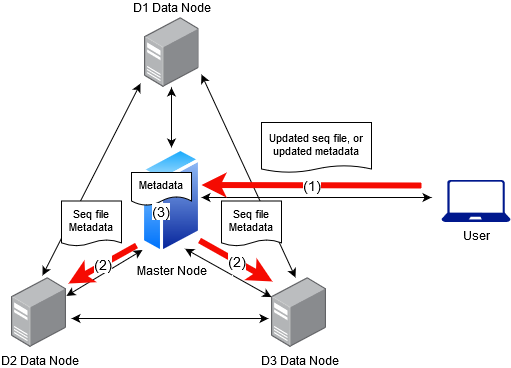
\includegraphics[width=0.80\linewidth]{images/thesis1-Page-5.png} 
\end{Figure}

\begin{Figure}
\captionof{figure}{DELETE: Deleting a sequence}
\centering
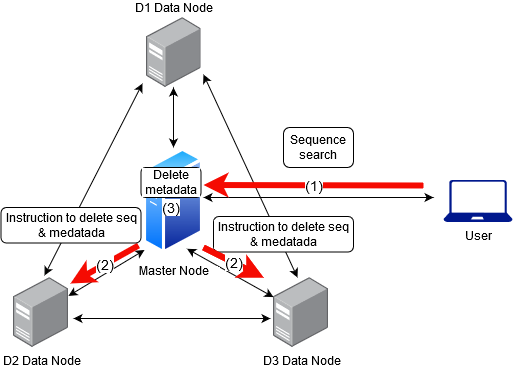
\includegraphics[width=0.80\linewidth]{images/thesis1-zzzzz.png} 
\end{Figure}

\begin{table*}[ht]
\caption{Data Model to be Used in the System}
\label{table:data_model_table}
\begin{tabular}{cl}
    \toprule
    key & description \\
    \midrule
    seq\textunderscore id & unique ID assigned to all sequences \\
    organism & organism where the sequence was extracted from \\
    quality & the rating of the data based on the number of downloads or another criteria \\
    uploader & user that uploaded the data \\
    institute & institute where the uploader or sequence was taken from \\
    upload\textunderscore date & date the data was uploaded to the database \\
    last\textunderscore modified & the date the metadata or data was edited \\
    data\textunderscore nodes & list of data nodes that this data is contained to \\
    \bottomrule
\end{tabular}
\end{table*}

Table~\ref{table:data_model_table} aims to show the metadata that will be initially stored in the database.

%CID: Data Permissions
\begin{table*}[ht]
\caption{Data Permissions and Users in the System}
\label{table:data_perm_table}
\begin{tabular}{cl}
    \toprule
    user & description \\
    \midrule
   Moderator & Has ability to upload, download, verify \\
    Registered User & Has ability to upload, download \\
    Guest & Has ability to download \\
   \bottomrule 
\end{tabular}
\end{table*}

Table~\ref{table:data_perm_table} shows the different set of users and the permissions allowed to them in the system. The moderator is a special user who has the ability to not allow some data to be uploaded. This is to make sure there is a means to verifying the data being uploaded. All registered users can upload and download. All other users, which are called guests, have an ability to download data.


\subsection{Community Aspect} \label{community}
The system was also described as community assisted. The definition of \textbf{community} to be used here is a \textit{set of people and institutions who generally collaborate together to do research}. And the focus is the genome research community. Reemphasizing certain features from the database, that any registered user can upload data. This means all users in the community can contribute to the knowledge base, and contribute data to be used by the community. Another important community aspect is that institutions can increase the number of data nodes. Meaning there will be an increase in the overall storage of the database, and at the same time theoretically increase data speeds (which will be discussed more later). Frequently used local data as well will be more easily accessible (since data nodes should have faster access speeds). The concept of closer networks having faster speeds (discussed in the network section) is at play here. Another community aspect will be this paper, publicly describing many aspects of the structure and code. So that this concept may be further developed and even implemented by genome research communities.

To summarize, this helps the community since the community may add their own data. The community may increase storage (through data nodes) these may also assist in increasing data speeds. And frequently used data will have faster access. 



\section{Proof of Correctness}
The distributed database will function correctly if:

\begin{enumerate}
    \item GET transfers the data to the user with no error
    \item POST transfers the data to the data node with no error
    \item PUT edits the data
    \item DELETE removes the data
    \item all DATA NODES with DATA X have the exact copy of DATA X
\end{enumerate}


The system will function correctly if it fulfills the main APIs without error, and that it is able to be partition-tolerant. Meaning the data is synchronized between the nodes. A proof of correctness for the implementation.

\section{Theoretical Analysis of Speed} 

Theoretical analysis of the speed up by checking time complexity of the base method versus the proposed method.

\subsection{Base Method}
In the base method, represented by NCBI (see Section \ref{NCBI}). We will abstract the transfer into this algorithm. Assuming as well, constant speed, equal division of bandwidth, all users are getting the same data all at once, and there is a constant overhead before downloading can occur.

\subsubsection{Base Method Algorithm}
\begin{enumerate}
    \item There is a constant overhead H seconds to set up the communication between the user and the main server.
    \item The main server sends data in the speed of X bytes per second. X is the speed of data transfer from the server.
    \item Users will receive the data with an equal portion of the X bytes per second (bandwidth).
\end{enumerate}

\subsubsection{Base Case of the Base Method}
    \begin{itemize} 
        \item 1 total users will receive data in the speed of X/1 bytes per second. Downloading data (size of X bytes) will take X/X + H seconds to transfer.
        \item 2 total users will receive data in the speed of X/2 bytes per second. Downloading data (size of X bytes) will take X/(2X) + H seconds to transfer.
    \end{itemize}

\subsubsection{General Case of the Base Method} 
With simple induction we can assume the general case to be: N total users will receive data in the speed of X/N bytes per second, with H seconds of an initial overhead. N is the number of users sharing the bandwidth. Downloading data (size of X bytes) will take X/(NX) + H or (1/N) + H seconds to transfer. A notable aspect of this general case is that an increase in the number of users decreases the user download speed.

\subsubsection{Notable Cases of the Base Method}
    \begin{itemize} 
        \item If N = X, all users will receive data with 1 byte per second.
        \item If N > X, all users will receive data with less than 1 byte per second, or if we forego the assumption of total equal division: Some will receive 1 byte per second, and others will receive 0 bytes per second or no transfer at all. This a bottleneck scenario.
    \end{itemize}

\subsection{Proposed Method}
For the proposed system, it is very similar to the base method, but the idea of data nodes (D) will be introduced. We will abstract the system into this algorithm. Assuming as well, constant speed, equal division of bandwidth, all users are getting the same data as once, there is a constant overhead before downloading the data for each user, there is also an equal division of the data nodes' bandwidth to the users, and all data nodes have an exact copy of the data.

\subsubsection{Proposed Method Algorithm for One Data Node}

\begin{enumerate}
    \item There is a constant overhead H seconds to set up the communication between the user and the relevant nodes.
    \item One data node will send data in the speed of X bytes per second. X is the speed of data transfer from 1 data node.
    \item Users will receive data with an equal portion of the X bytes per second. 
\end{enumerate}

\subsubsection{Base Case of the Proposed Method for One Data Node}

\begin{itemize} 
    \item 1 total user (and 1 data node) will receive data in the speed of 1 times X/1 bytes per second. Downloading data (size of X bytes) will take X/X + H seconds to transfer.
    \item 2 total users (and 1 data node) will receive data in the speed of 1 times X/2 bytes per second. Downloading data (size of X bytes) will take X/(2X) + H seconds to transfer.
\end{itemize}


\subsubsection{General Case of the Proposed Method for One Data Node} 
Exactly the same as the  General Case of the Base Method, N total users and 1 data node will receive data in the speed of X/N bytes per second with H seconds of an initial overhead. N is the number of users sharing the bandwidth. Downloading data (size of X bytes)  will take X/(NX) + H or (1/N) + H seconds to transfer.

\subsubsection{Proposed Method Algorithm for Multiple Data Nodes}
\begin{enumerate}
    \item There is a constant overhead H seconds to set up the communication between the user and the relevant nodes.
    \item All data nodes (D number of data nodes) will send data in the speed of D times X bytes per second. X is the speed of data transfer from 1 data node.
    \item Users will receive data with an equal portion of the D times X bytes per second.
\end{enumerate}


\subsubsection{Base Case of the Proposed Method for Multiple Data Nodes}
\begin{itemize}
    \item 1 total users (and D data nodes) will receive data in the speed of D times X/1 bytes per second. Downloading data (size of X bytes) will take DX/X + H seconds to transfer.
    \item 2 total users (and D data nodes) will receive data in the speed of D times X/2 bytes per second. Downloading data (size of X bytes) will take DX/(2X) + H seconds to transfer.
\end{itemize}




\subsubsection{General Case of the Proposed Method for Multiple Data Nodes} 
This is different from the General Case of the Proposed Method for a Single Data Node by a factor of D. N total users and D data nodes will receive data in the speed of DX/N bytes per second with H seconds of an initial overhead. N is the number of users sharing the bandwidth. Downloading data (size of X bytes)  will take DX/(NX) + H or (D/N) + H seconds to transfer. A notable aspect of this general case is that as the number of data nodes increases, the user's speed also increases. Even if the previous feature from the general case of the base method is still at play, (an increase in the number of users decreases the user download speed).

\subsubsection{Notable Cases of the Proposed Method}
\begin{itemize}
    \item  If D = 1, N = X, all users will receive data with 1 byte per second (base method and proposed method for one data node is excactly the same).
    \item If D = 1, N > X, all users will receive data with less than 1 byte per second, or if we forego the assumption of total equal division: Some will receive 1 byte per second, and others will receive 0 bytes per second or no transfer at all. This a bottleneck scenario. (also the same).
    \item If D = 0, there is no data transfer at all. This is an extreme case.
    \item If D = 1, the proposed method will match the base case, general cases, and notable cases for the base method
    \item If D > 1, the proposed method will be faster than the base method (as long as H, X, N are the same).
\end{itemize}

\subsection{Summary of the Theoretical Analysis of Speed} \label{theoreticalspeed}
Generally as the number of users increases, the data transfer speed decreases by a constant factor for all methods. There is also a concept of bottleneck when the number of users is much greater than the data speed put out by all methods.

The proposed method (with D > 1, and same H, X, N) will be faster than the base method. A notable extreme for the proposed method is that once D = 0, no transfer will occur and will be slower than the bottleneck base method. With this analysis, it is suggested the proposed method is faster than the base method on most cases (D > 1). 

\section{Comparison of base method vs proposed method}

For the final comparisons of the base method the proposed method, the current base method (NCBI in Section \ref{NCBI}) is the go-to website for biological data and genomic data. It is currently used and is one website and one server. This points to a single point of failure\cite{seqtorr}. The section \ref{theoreticalspeed} on theoretical analysis of speed described the problem of having a bottleneck when the number of users are too many for the data bandwidth of the server. 

The proposed method introduces the idea of data nodes and in section \ref{theoreticalspeed} explains how having at least one data node should theoretically rival the speed of the base method. And having multiple data nodes will be faster in theory than the base method. Another advantage of having a distributed database is the community aspect (see Section \ref{community}). The proposed method may be implemented on a local scale, meaning it can have the necessary data for the community. The most frequently used data, may be put on more data nodes increasing the speed of the data transfer (see Section \ref{theoreticalspeed}). Another is that the features on the designs of the speed, consistency, and fault tolerance  may be calibrated to the needs of the community. 

\section{Conclusion}
The research designed a theoretical design for a database for genomics researchers. The database is distributed and uses a hybrid architecture when managing the data. The theoretical properties of the design was studied and compared to a base method (FTP of NCBI), notably the speed and correctness. The proposed system, is better suited for database systems that scale. And is shown to be faster if there are multiple data nodes.

\section{Recommendations}
A recommendation is to implement this proposed system. It is advised to have a public code with an easy-to-start documentation.

A small but important technical step is to pay attention to port access especially with university internet, some universities only limit the usable ports to two and this would be an important hurdle to overcome in managing multiple data nodes.

Another is to look into security. How does data privacy work? And how does security affect the accessibility of the system? What are the different risks in distributed databases and how to prevent them? Many questions arise in security but these will only be answered better once implementation starts.

The last recommendation is to abstract this project for non-genomic data as well. This is good especially for other scientific communities with its own growing data set such as cosmology with its space image data. 

%%%%%%%%%%%%%%%%%%%%%%%%%%%% ACKNOWLEDGEMENT & GRATITUDE %%%%%%%%%%%%%%%%%%%%%%%%%%%%%%%
%%
%% The acknowledgments section is defined using the "acks" environment
%% (and NOT an unnumbered section). This ensures the proper
%% identification of the section in the article metadata, and the
%% consistent spelling of the heading.
\begin{acks}

We want to acknowledge our advisers Dr. Jan Michael Yap and Sir El King Morado for giving the idea for our thesis. They have answered our many questions about genomics. Writing this paper overlapped with the covid19 pandemic which changed a big portion of the scope of this thesis. We have unexpressable gratitude to our advisers for being understanding and trusting with this. We also thank the people from Philipping Genome Center who welcomed us and gave us coffee and a workstation.
\end{acks}

%%
%% The next two lines define the bibliography style to be used, and
%% the bibliography file.
%\bibliographystyle{ACM-Reference-Format}
\bibliographystyle{newapa}
\bibliography{bibfile}



\end{multicols}{2}

\end{document}
\endinput
%%
%% End of file `sample-acmsmall.tex'.
%%

\bibliography{bibfile}

